\documentclass[12pt,a4paper]{article}
\author{Wannes {De Craene} \and Michiel Schoofs \and Lieven {Van Loo} \and Wannes Sergeant}
\title{Literatuurstudie - Paper Onderzoekstechnieken}
\date{\today}
\usepackage[dutch]{babel}

\usepackage{graphicx}
\graphicspath{{./grafieken/}}

\usepackage{nameref}
\usepackage{subcaption}
%new command section
\newcommand{\customref}[1]{\underline{\ref{#1}: \nameref{#1}}}

\usepackage[backend=biber,style=apa]{biblatex}
\addbibresource{bibliografie.bib}

\begin{document}
    
    \maketitle
    
    \tableofcontents

    \newpage
    \section{Inleiding}
    
    Voor ons onderzoek over Retrieval Practice hebben wij eerst een literatuurstudie gemaakt om duidelijk uit te lijnen wat wij juist verwachten van het experiment zelf.
    \subsection{Variabelen}
    Concreet hebben wij beslist om een extra variabelen te gaan introduceren namelijk de geheugen capaciteit van het proefpubliek. Ook hebben wij beslist om de retentie test te hervormen volgens twee principes: Rote en Meaningful Learning (lees als uit het hoofd leren en kunnen toepassen).\\
    \par
	\noindent    
    Verder delen we de proefpersonen op in drie delen, idem aan het originele experiment door \cite{HenryRoediger2006}, Deze zijn: Study-Study-Study-Study, Study-Study-Study-Test  en Study-Test-Test-Test. 
    \subsection{Verwachte conclusies}
    
    \section{Methodologie}
    \label{methodology}
    Om bovenstaande variabelen te kunnen gebruiken in onze conclusies moeten we ook uitlijnen hoe we deze willen gaan testen. Onder deze sectie vindt u een voorstel over hoe we deze verschillende variabelen op een empirische manier zouden kunnen meten.
    
	    \subsection{Meten van geheugencapaciteit}
	    \label{methodology-gc}
	    Naar aanleiding van het artikel van \cite{Agarwal2016} gaan we onderzoeken of er een correlatie is tussen de geheugencapaciteit en de doeltreffendheid van Retrieval Practice. -Voor meer informatie zie ook sectie \customref{geheugencapaciteit}.- We moeten echter eerst verduidelijken hoe we deze capaciteit zouden gaan meten in onze testgroepen.\\
	    \par
	    \noindent
	    We kunnnen gebruik maken van een woordenlijst van 25 woorden elk toenemend in lengte. De proefpersoon in kwestie krijgt 5 minuten om de woordenlijst te memoriseren en wordt vervolgens gevraagd om deze te reproduceren.Daarna wordt een score toegekend volgens volgend principe: Een volledig correct geschreven woord krijgt 2 punten, een woord dat fonetisch correct is krijgt 1 punt.\\
	    \par
	    \noindent
	    Door deze methode te hanteren zijn we instaat om de groep in twee delen op te splitsen. De groep die hoger scoorde dan de mediaan bestempelen we als \textit{Hoge geheugencapaciteit} de overige groep benoemen we als \textit{Lage geheugencapaciteit}
	    
      	\subsection{Hervorming van de retentie test}
      	We gaan eveneens de retentie test veranderen. Dit doen we naar aanleiding van het artikel geschreven door \cite{TamaravanGog2012}. Concreet willen we het type van memorisatie (ROTE of Meaningful) door Retrieval Practice gaan bestuderen. -Voor meer informatie zie sectie \customref{RoteVSMeaningful}.-\\
      	
      	\par
      	\noindent
      	
    \newpage
    \section{Literatuurstudie}
    
    Voor we kunnen van start gaan met het onderzoek moeten we eerst een literatuurstudie schrijven om duidelijk uit te lijnen wat we precies verwachten. We geven dus wat meer uitleg rond het algemene doel van ons experiment en de gekozen variabelen.
    
        \subsection{Onderscheid in geheugen capaciteit}
        \label{geheugencapaciteit}
        Vooraleer het experiment van start gaat hebben wij beslist om een onderscheid te maken tussen groepen met een verschillende geheugencapaciteit, dit omdat wij, na het lezen van een artikel omtrent geheugencapaciteit van \cite{Agarwal2016} het vermoeden hebben dat de invloeden van retrieval practice verschillen bij mensen met een lagere (of hogere) geheugencapaciteit.
                
        \subsection{Wat is Leren?}
        
        \subsection{Rote vs Meaningful Learning}
        \label{RoteVSMeaningful}
        
        \subsection{Retrieval Practice}
        
        Wat verstaan we nu juist onder het systeem ``Retrieval Practice''? Concreet is dit een systeem waarbij je leerstof gaat leren door het afnemen van testen, in de plaats van gewoon een boek te nemen en het op conventionele wijze te gaan studeren.
        
            \subsubsection{Invloed Feedback op Retrieval Practice}
            
            Het belangrijkste element van retrieval practice is het testen, maar feedback op die testen mogen we zeker niet negeren. We hebben echter geleerd uit \cite{HenryRoediger2011} dat feedback zeker niet te verwaarlozen is. Het verschil tussen wel en geen feedback is best groot: in het geval van hun onderzoek waren de resultaten 30\% tot 64\% beter, afhankelijk van op welk moment de feedback gebeurde, namelijk direct na de test of met enige tijd ertussen. 
    
            \subsubsection{Invloed Vertrouwen met de stof op de prestatie}
            
            De voorkennis op de leerstof is een belangrijke factor voor het studeren, en kan ook 
            belangrijk zijn voor het kiezen van een leerstrategie. Zo toont \cite{Xiaofeng2016} aan dat voorkennis een minder bepalende factor is bij retrieval practice dan bij elaboration, waarbij studenten de nieuwe informatie verwerken door middel van relaties te trekken met gekende leerstof.
            Bij elaboration hadden studenten met ruimere voorkennis een groot voordeel, terwijl bij retrieval
            practice de voorkennis geen bepalende factor was.
            Studenten die niet gekend zijn met de leerstof kunnen volgens ons dus beter voor retrieval 
            practice kiezen.
            
        \subsection{Addendum}
        
        Verder hebben we nog enkele artikels die zeer nuttige info bevatten, maar die niet absoluut noodzakelijk zijn voor het succesvol af te werken van het experiment, daarom hebben wij deze dus ter info nog toegevoegd.
        
        \subsubsection{Successful inhibition, unsuccessful retrieval: Manipulating time and success during retrieval practice}
        
        Hier spreekt men eigenlijk over exact hetzelfde als ons, maar op een omgekeerde wijze. Wat bedoelen we hier juist mee? Wel, in het vooraf uitgevoerde experiment van \cite{HenryRoediger2006} teste men op het behouden van informatie, in dit artikel van \cite{BenjaminStorm2009} bekeek men wat de proefpersonen vergaten. Dit is dus niet echt noodzakelijk artikel, maar het blijkt wel interessant om te zien dat het omgekeerde experiment tot een quasi idem resultaat leid. Dit artikel werd geschreven door. 
        
        \subsubsection{Commentary: Retrieval practice protects memory against acute stress}
        
        In dit artikel van \cite{Smith2016} bekijkt men welke invloed ``Retrieval Practice'' heeft op stress, terwijl dit wel een goede variabele zou zijn om op te nemen in dergelijke onderzoeken hebben wij beslist om onze focus ergens anders te leggen.
        
        \subsubsection{Optimizing retrieval as a learning event: When and why expanding retrieval practice enhances long-term retention}
        
        Dit artikel, geschreven door \cite{Storm2010} is zo goed als een ``kopie'' van het voorafgenoemde artikel van \cite{HenryRoediger2006}, dit kunnen we dus ook niet echt opnemen in onze studie, maar het is handig om te zien dat er een volledig losstaand onderzoek tot een zeer gelijkaardig resultaat komt. 
        
        \subsubsection{Retrieval Practice Produces More Learning than Elaborative Studying with Concept Mapping}
        
        Aangezien men spreekt over een nieuwe studiemethode was het ook interessant om te bekijken of er nu nog andere methodes dan enkel Retrieval Practice zijn die bevorderend werken voor de retentie van geziene leerstof. \cite{JeffreyKarpicke2011} voegt hier een extra studiemethode genaamd ``Concept Mapping'' uit, dit had dus ook een leuke variabele kunnen zijn voor ons onderzoek, maar zoals voordien vermeld zijn wij een andere weg op gegaan.
    
    \newpage
    \section{Mock Grafieken}
    
    	\subsection{Duiding}
    	
    	Analoog aan de artikels van \cite{HenryRoediger2006} en \cite{Agarwal2008}, zullen we gebruik maken van zowel grafieken als tabellen om onze hypotheses te staven. Op deze manier kunnen we de gebruikte dataset vereenvoudigen en op een compacte en correcte manier conclusies gaan trekken.\\
    	\par
    	\noindent
    	We zouden graag toch een moment nemen om stil te staan bij de verschillende variabelen en veronderstellingen die we gebruiken om deze grafieken te maken. Zo hopen we foutieve communicatie te voorkomen.
    	
    	\subsection{Grafieken}
    	
    	\subsubsection{Uitleg}
    	De grafieken die we gebruiken zijn opgedeeld in twee groepen (uitgeleind in sectie \customref{methodology-gc}):
    	\begin{itemize}
    		\item De groep met een \textit{lage geheugencapaciteit (LGC)}: Dit is de testgroep die op de voorafgenomen woordenlijst onder de mediaan scoorde. Deze testgroep zit dus met andere woorden in de laagste 50\% van de afgenomen testen betreffende hun score.
    		\item De groep met een \textit{hoge geheugencapaciteit (HGC)}: Dit is de groep die boven de mediaan scoorde. Kortom de groep die bij de hoogste 50\% zit qua hun score op de woordenlijst.
    	\end{itemize}
    
    	\newpage
    	\subsubsection{Grafieken} 
		\begin{figure}[h]
			\begin{subfigure}{0.6\textwidth}
				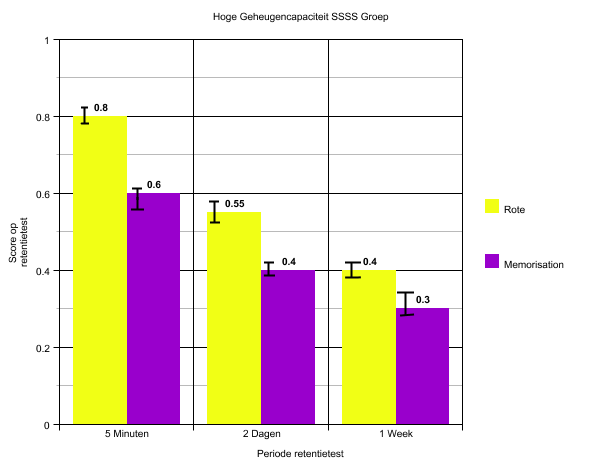
\includegraphics[width=\linewidth]{grafiek1}
				\caption{HGC Grafiek SSSS}
			\end{subfigure}
			\begin{subfigure}{0.6\textwidth}
				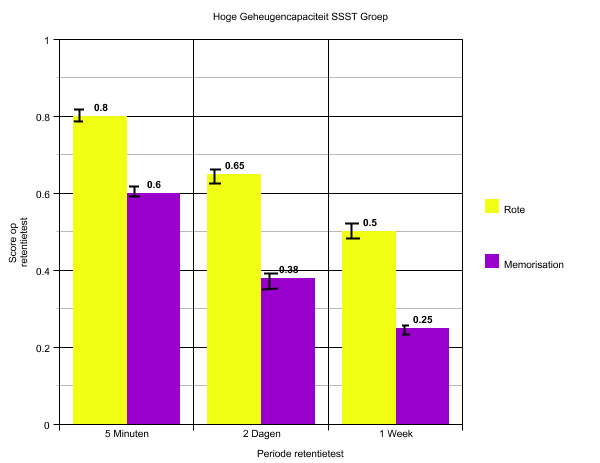
\includegraphics[width=\linewidth]{grafiek3}
				\caption{HGC Grafiek SSST}
			\end{subfigure}
			\begin{subfigure}{0.6\textwidth}
				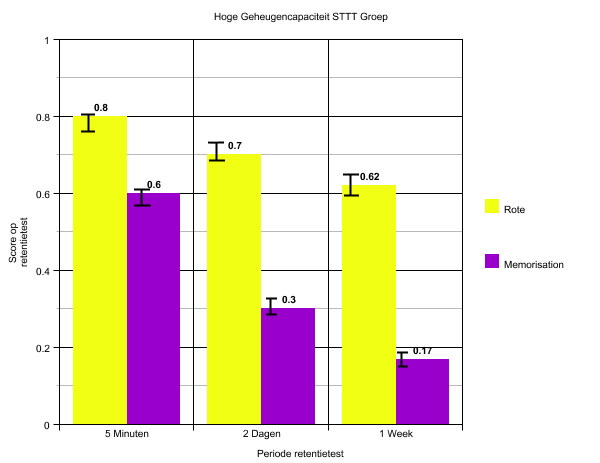
\includegraphics[width=\linewidth]{grafiek5}
				\caption{HGC Grafiek STTT}
			\end{subfigure}
			\caption{Grafieken van de Hoge Geheugencapaciteit groep}
		\end{figure}
    \newpage
    \section{Referenties}
    
	\printbibliography
    
\end{document}